%        File: algorithm.tex
%     Created: Wed Dec 30 02:00 PM 2009 S
% Last Change: Wed Dec 30 02:00 PM 2009 S
%
\documentclass[a4paper]{article}
\usepackage[top=1in, bottom=1in, left=0.5in, right=0.5in]{geometry}
%\usepackage[lined, boxed, commentsnumbered, oldcommands]{algorithm2e}
\usepackage[lined, boxed, commentsnumbered]{algorithm2e}
\usepackage{graphicx}
\usepackage{multicol}
\begin{document}

\section{Routings in transformation program}

\begin{algorithm}[H]
\SetLine
\linesnumbered
\dontprintsemicolon
\SetKwData{Program}{program}
\SetKwData{NewProgram}{new\_program}
\SetKwData{Block}{block}
\SetKwData{NewBlock}{new\_block}
\SetKwData{Statement}{statement}
\SetKwData{Evalprog}{eval\_prog}
\SetKwData{Constant}{constant}
\SetKwData{ConstantPool}{constant\_pool}
\SetKwData{CT}{CT}
\SetKwData{CTVal}{CT\_val}
\SetKwData{Pointer}{pointer}
\SetKwData{Val}{val}
\SetKwData{Pointers}{pointers[ ]}
\SetKwData{AST}{ast}
\SetKwFunction{MixProg}{Mix\_Program}
\SetKwFunction{BuildConstantTrees}{build\_constant\_trees}
\SetKwFunction{Decode}{decode}
\SetKwFunction{Append}{append}
\SetKwFunction{Substutite}{substutite}
\SetKwFunction{HaveConstant}{have\_constant}
\SetKwFunction{LocateSubtree}{locate\_subtree}
\SetKwFunction{UpdateGraph}{update\_graph}
\SetKwFunction{DynamicBuildConstantTree}{dynamic\_build\_constant\_tree}
\SetKwInOut{Input}{input}
\SetKwInOut{Output}{output}

\Input{\Program, program to be processed; \AST, abstact syntax tree of the program}
\Output{\NewProgram, processed program}

\BlankLine  
\NewProgram $\leftarrow \emptyset$\; 
\ForEach{\Block $\in$ \Program}
{
    \NewBlock $\leftarrow \emptyset$ \;
    \Pointers $\leftarrow \emptyset$ \;
    \BlankLine 
    \Evalprog $\leftarrow$ Construct a random evaluation program
                           from the evaluation templates \;
    \Block $\leftarrow$ \MixProg{\Block, \Evalprog} \;
    \ConstantPool $\leftarrow$ [All constants in the block] \;
    \CT $\leftarrow$ \BuildConstantTrees{\ConstantPool, \Pointers} \;
    \CTVal $\leftarrow$ \Decode{\CT}\;
    \Append{\NewBlock, \DynamicBuildConstantTree{\CTVal}} \;
    \BlankLine  
    \ForEach{\Statement $\in$ \Block} 
    {
        \If{\HaveConstant{\Statement, \AST}}
        {
            \ForEach{\Constant $\in$ \Statement}
            {
                \Pointer $\leftarrow$ \LocateSubtree{\Pointers, \Constant} \;
                \Substutite{\Statement, \Constant, \Decode{\Pointer}} \;
            } \;
        } \;
        \Val $\leftarrow$ left value of the statement \;
        \Append{\NewBlock, \Statement}\;
        \Append{\NewBlock, \UpdateGraph{\CT, \Val}} \;
    } \;
    \Append{\NewProgram, \NewBlock}\;
} \;
 
\BlankLine 
\Return{\NewProgram}\;
\caption{Overview}
\end{algorithm}

\begin{algorithm}
\SetLine
\linesnumbered
\dontprintsemicolon
\SetKwData{Constant}{constant}
\SetKwData{Pointers}{pointers[ ]}
\SetKwData{Pointer}{pointer}
\SetKwInOut{Input}{input}
\SetKwInOut{Output}{output}

\Input{\Constant, constant to be search in the tree\\
       \Pointers, a set of pointers used to point to the\\
       root of the subgraphs representing the constant}
\Output{\Pointer, the root of the subgraph representing the constant\\
       $NULL$, if not find}

       \BlankLine
       \eIf{\Constant $\in$ \Pointers}
       {
            \Return \Pointer\;
       }
       {
            \Return $NULL$ \;     
       }
\caption{Locate subtree}
\end{algorithm}


\begin{algorithm}[H]
\SetLine
\linesnumbered
\dontprintsemicolon
\SetKwData{CT}{CT}
\SetKwData{Constant}{constant}
\SetKwData{ConstantPool}{constant\_pool}
\SetKwData{Pointers}{pointers[ ]}
\SetKwData{SubtreeRoot}{subtree\_root}
\SetKwData{Node}{node}
\SetKwData{InitTree}{init\_tree}
\SetKwFunction{BuildConstantTree}{build\_const\_tree}
\SetKwFunction{RandomNode}{random\_node}
\SetKwFunction{MergeTree}{merge\_tree}
\SetKwFunction{LocateSubtree}{locate\_subtree}
\SetKwFunction{FJoin}{join}
\SetKwInOut{Input}{input}
\SetKwInOut{Output}{output}
\Input{\ConstantPool, a set of constants used in the block;\\
       \Pointers, a set of pointers used to point to the\\
       root of the subgraphs representing the constant}
\Output{\CT, the root of the constant tree}

\BlankLine
\CT $\leftarrow$ Root of \InitTree \;
\ForEach{\Constant $\in$ \ConstantPool}
{
    \SubtreeRoot $\leftarrow$ \BuildConstantTree{\Constant}\;
    \Node $\leftarrow$ \LocateSubtree{\Pointers, \Constant}\;
    \eIf(//if cannot find one, construct one){ \Node $==  NULL$}
    {
        \Node $\leftarrow$ \RandomNode{\CT}\;
        \MergeTree{\Node, \SubtreeRoot}\;
    }
    (//if find one, make a duplication in probability){
        toss a coin\;
        \If{head is up}
        {
            \Node $\leftarrow$ \RandomNode{\CT}\;
            \MergeTree{\Node, \SubtreeRoot}\;
        }\;
    }\;
    \Pointers.\FJoin{$($\Node, \Constant$)$}\;
}\;  

\Return{\CT}\;
\caption{Build Constant Trees}
\end{algorithm}

\section{Routings in watermarked program}

\begin{algorithm}[H]
\SetLine
\linesnumbered
\dontprintsemicolon
\SetKwData{CT}{CT}
\SetKwData{Node}{node}
\SetKwData{Left}{left}
\SetKwData{Right}{right}
\SetKwData{Parent}{parent}
\SetKwData{ParentPoint}{parent\_point}
\SetKwData{NewNode}{new\_node}
\SetKwData{AnotherNewNode}{another\_new\_node}
\SetKwData{Pointers}{pointers[ ]}
\SetKwData{Val}{val}
\SetKwFunction{FindUpgradableNode}{find\_upgradable\_node}
\SetKwFunction{Update}{update}
\SetKwFunction{NodeAllocate}{allocate}
\SetKwFunction{LeftRotatea}{left\_rotate\_1}
\SetKwFunction{LeftRotateb}{left\_rotate\_2}
\SetKwFunction{LeftRotatec}{left\_rotate\_3}
\SetKwFunction{LeftRotated}{left\_rotate\_4}
\SetKwFunction{RightRotatea}{right\_rotate\_1}
\SetKwFunction{RightRotateb}{right\_rotate\_2}
\SetKwFunction{RightRotatec}{right\_rotate\_3}
\SetKwFunction{RightRotated}{right\_rotate\_4}
\SetKwInOut{Input}{input}
\SetKwInOut{Output}{output}

\Input{\CT, the root of the constant tree; \Val, value update refers to}
\Output{None}

\BlankLine
\Node $\leftarrow$ \FindUpgradableNode{\CT}\;

\eIf{\Node $==$ \Node$\rightarrow$\Parent$\rightarrow$\Left}
{
    \ParentPoint $\leftarrow$ $\&$\Node$\rightarrow$\Parent$\rightarrow$\Left\;
}
{
    \ParentPoint $\leftarrow$ $\&$\Node$\rightarrow$\Parent$\rightarrow$\Right\;
}

\BlankLine
\eIf(//left rotate){val is odd}
{
    \Switch{rotate case}
    {
    \lCase{1}{\LeftRotatea{}} \;
    \lCase{2}{\LeftRotateb{}} \;
    \lCase{3}{\LeftRotatec{}} \;
    \lCase{4}{\LeftRotated{}} \;
    }
}
{
    \Switch{rotate case}
    {
    \lCase{1}{\RightRotatea{}} \;
    \lCase{2}{\RightRotateb{}} \;
    \lCase{3}{\RightRotatec{}} \;
    \lCase{4}{\RightRotated{}} \;
    } \;
} \;

\BlankLine
\If(//update the child pointers of the root){\CT$\rightarrow$\Left $\neq$ \CT$\rightarrow$\Right}
{
    \CT$\rightarrow$\Right $\leftarrow$ \CT$\rightarrow$\Left\;
}\;
\caption{UpdateGraph}
\end{algorithm}

\begin{algorithm}[H]
\SetKwData{Node}{node}
\SetKwData{Left}{left}
\SetKwData{Right}{right}
\SetKwData{Parent}{parent}
\SetKwData{ParentPoint}{parent\_point}

*\ParentPoint $\leftarrow$ \Node$\rightarrow$\Right\;
\Node$\rightarrow$\Right$\rightarrow$\Parent $\leftarrow$ \Node$\rightarrow$\Parent\;
\Node$\rightarrow$\Parent $\leftarrow$ \Node$\rightarrow$\Left\;
\Node$\rightarrow$\Right $\leftarrow$ \Node$\rightarrow$\Parent$\rightarrow$\Left\;
\Node$\rightarrow$\Parent$\rightarrow$\Left$\rightarrow$\Parent $\leftarrow$ \Node\;
\Node$\rightarrow$\Parent$\rightarrow$\Left $\leftarrow$ \Node\;
\caption{Left rotate case 1}
\end{algorithm}

\begin{algorithm}[H]
\SetKwData{Node}{node}
\SetKwData{Left}{left}
\SetKwData{Right}{right}
\SetKwData{Parent}{parent}
\SetKwData{ParentPoint}{parent\_point}
\SetKwData{NewNode}{new\_node}
\SetKwData{AnotherNewNode}{another\_new\_node}
\SetKwData{Pointers}{pointers[ ]}
\SetKwFunction{NodeAllocate}{allocate}
\SetKwFunction{Update}{update}

\NodeAllocate{\NewNode}\;
\NewNode$\rightarrow$\Left $\leftarrow$ \Node$\rightarrow$\Right$\rightarrow$\Left\;
\NewNode$\rightarrow$\Right $\leftarrow$ \Node$\rightarrow$\Right$\rightarrow$\Right\;
\Node$\rightarrow$\Right$\rightarrow$\Left$\rightarrow$\Parent $\leftarrow$ \NewNode\;
\Node$\rightarrow$\Right$\rightarrow$\Right$\rightarrow$\Parent $\leftarrow$ \NewNode\;
\Node$\rightarrow$\Right$\rightarrow$\Right $\leftarrow$ \NewNode\;
\Node$\rightarrow$\Right$\rightarrow$\Left $\leftarrow$ \Node\;
\Node$\rightarrow$\Right$\rightarrow$\Parent $\leftarrow$ \Node$\rightarrow$\Parent\;
*\ParentPoint $\leftarrow$ \Node$\rightarrow$\Right\;
\Node$\rightarrow$\Parent $\leftarrow$ \Node$\rightarrow$\Right\;
\NodeAllocate{\AnotherNewNode}\;
\Node$\rightarrow$\Right $\leftarrow$ \AnotherNewNode\;
\Pointers.\Update{\Node$\rightarrow$\Parent, \Node$\rightarrow$\Parent$\rightarrow$\Right}\;
\caption{Left rotate case 2}
\end{algorithm}

\begin{algorithm}[H]
\SetKwData{Node}{node}
\SetKwData{Left}{left}
\SetKwData{Right}{right}
\SetKwData{Parent}{parent}
\SetKwData{ParentPoint}{parent\_point}

$*$\ParentPoint $\leftarrow$ \Node$\rightarrow$\Left\;
\Node$\rightarrow$\Left$\rightarrow$\Parent $\leftarrow$ \Node$\rightarrow$\Parent\;
\Node$\rightarrow$\Parent $\leftarrow$ \Node$\rightarrow$\Right\;
\Node$\rightarrow$\Left $\leftarrow$ \Node$\rightarrow$\Parent$\rightarrow$\Right\;
\Node$\rightarrow$\Parent$\rightarrow$\Right$\rightarrow$\Parent $\leftarrow$ \Node\;
\Node$\rightarrow$\Parent$\rightarrow$\Right $\leftarrow$ \Node\;
\caption{Right rotate case 1}
\end{algorithm}

\begin{algorithm}[H]
\SetKwData{Node}{node}
\SetKwData{Left}{left}
\SetKwData{Right}{right}
\SetKwData{Parent}{parent}
\SetKwData{ParentPoint}{parent\_point}
\SetKwData{NewNode}{new\_node}
\SetKwData{AnotherNewNode}{another\_new\_node}
\SetKwData{Pointers}{pointers[ ]}
\SetKwFunction{NodeAllocate}{allocate}
\SetKwFunction{Update}{update}

\NodeAllocate{\NewNode}\;
\NewNode$\rightarrow$\Left $\leftarrow$ \Node$\rightarrow$\Right$\rightarrow$\Left\;
\NewNode$\rightarrow$\Right $\leftarrow$ \Node$\rightarrow$\Right$\rightarrow$\Right\;
\Node$\rightarrow$\Right$\rightarrow$\Left$\rightarrow$\Parent $\leftarrow$ \NewNode\;
\Node$\rightarrow$\Right$\rightarrow$\Right$\rightarrow$\Parent $\leftarrow$ \NewNode\;
\Node$\rightarrow$\Right$\rightarrow$\Right $\leftarrow$ \NewNode\;
\Node$\rightarrow$\Right$\rightarrow$\Left $\leftarrow$ \Node\;
\Node$\rightarrow$\Right$\rightarrow$\Parent $\leftarrow$ \Node$\rightarrow$\Parent\;
*\ParentPoint $\leftarrow$ \Node$\rightarrow$\Right\;
\Node$\rightarrow$\Parent $\leftarrow$ \Node$\rightarrow$\Right\;
\NodeAllocate{\AnotherNewNode}\;
\Node$\rightarrow$\Right $\leftarrow$ \AnotherNewNode\;
\Pointers.\Update{\Node$\rightarrow$\Parent, \Node$\rightarrow$\Parent$\rightarrow$\Right}\;
\caption{Right rotate case 2}
\end{algorithm}

\section{Routings shared in both parts}

\begin{algorithm}[H]
    \caption{Build Constant Tree}
\end{algorithm}

\begin{algorithm}[H]
    \caption{decode}
\end{algorithm}

\appendix
\begin{figure}
    \centering
    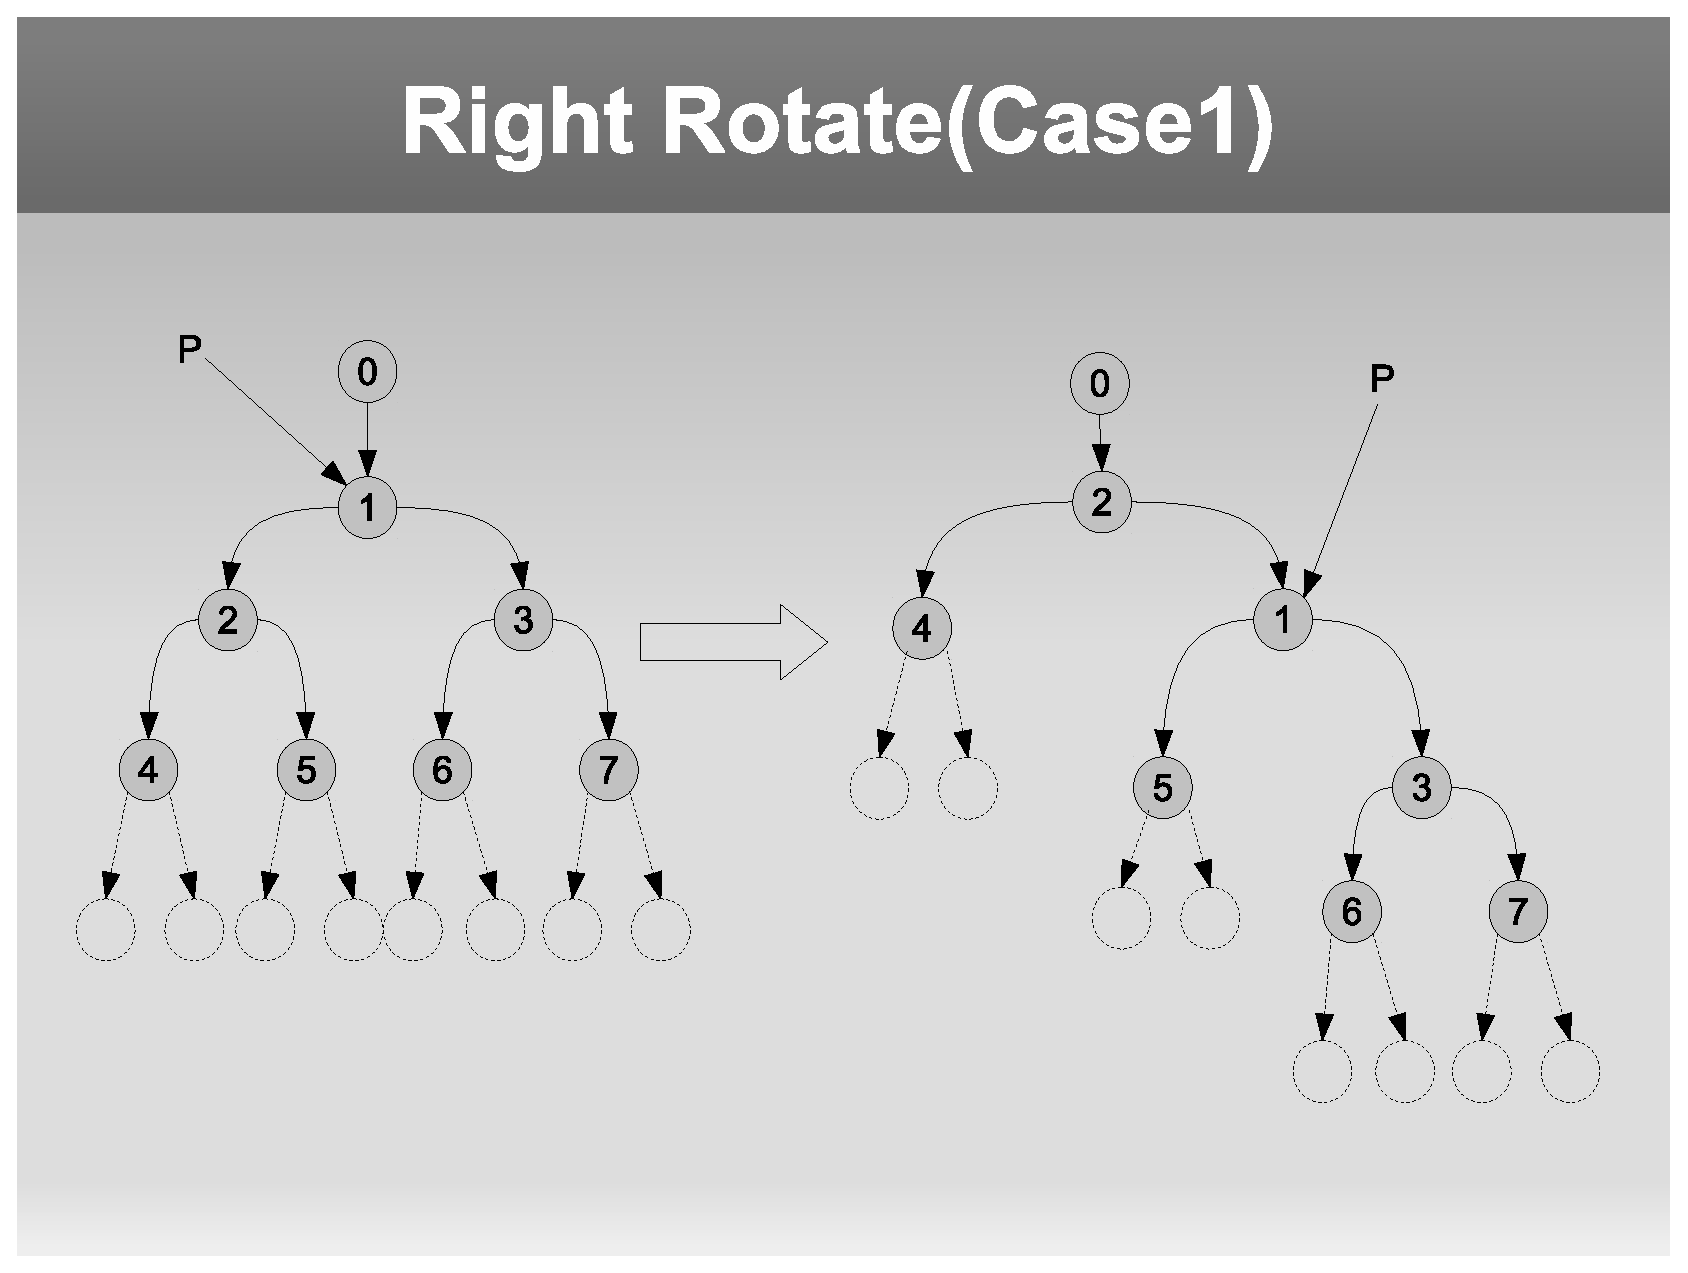
\includegraphics[scale=0.5]{right_rotate_1.eps}
    \caption{Right Rotate Case 1}
\end{figure}

\begin{figure}
    \centering
    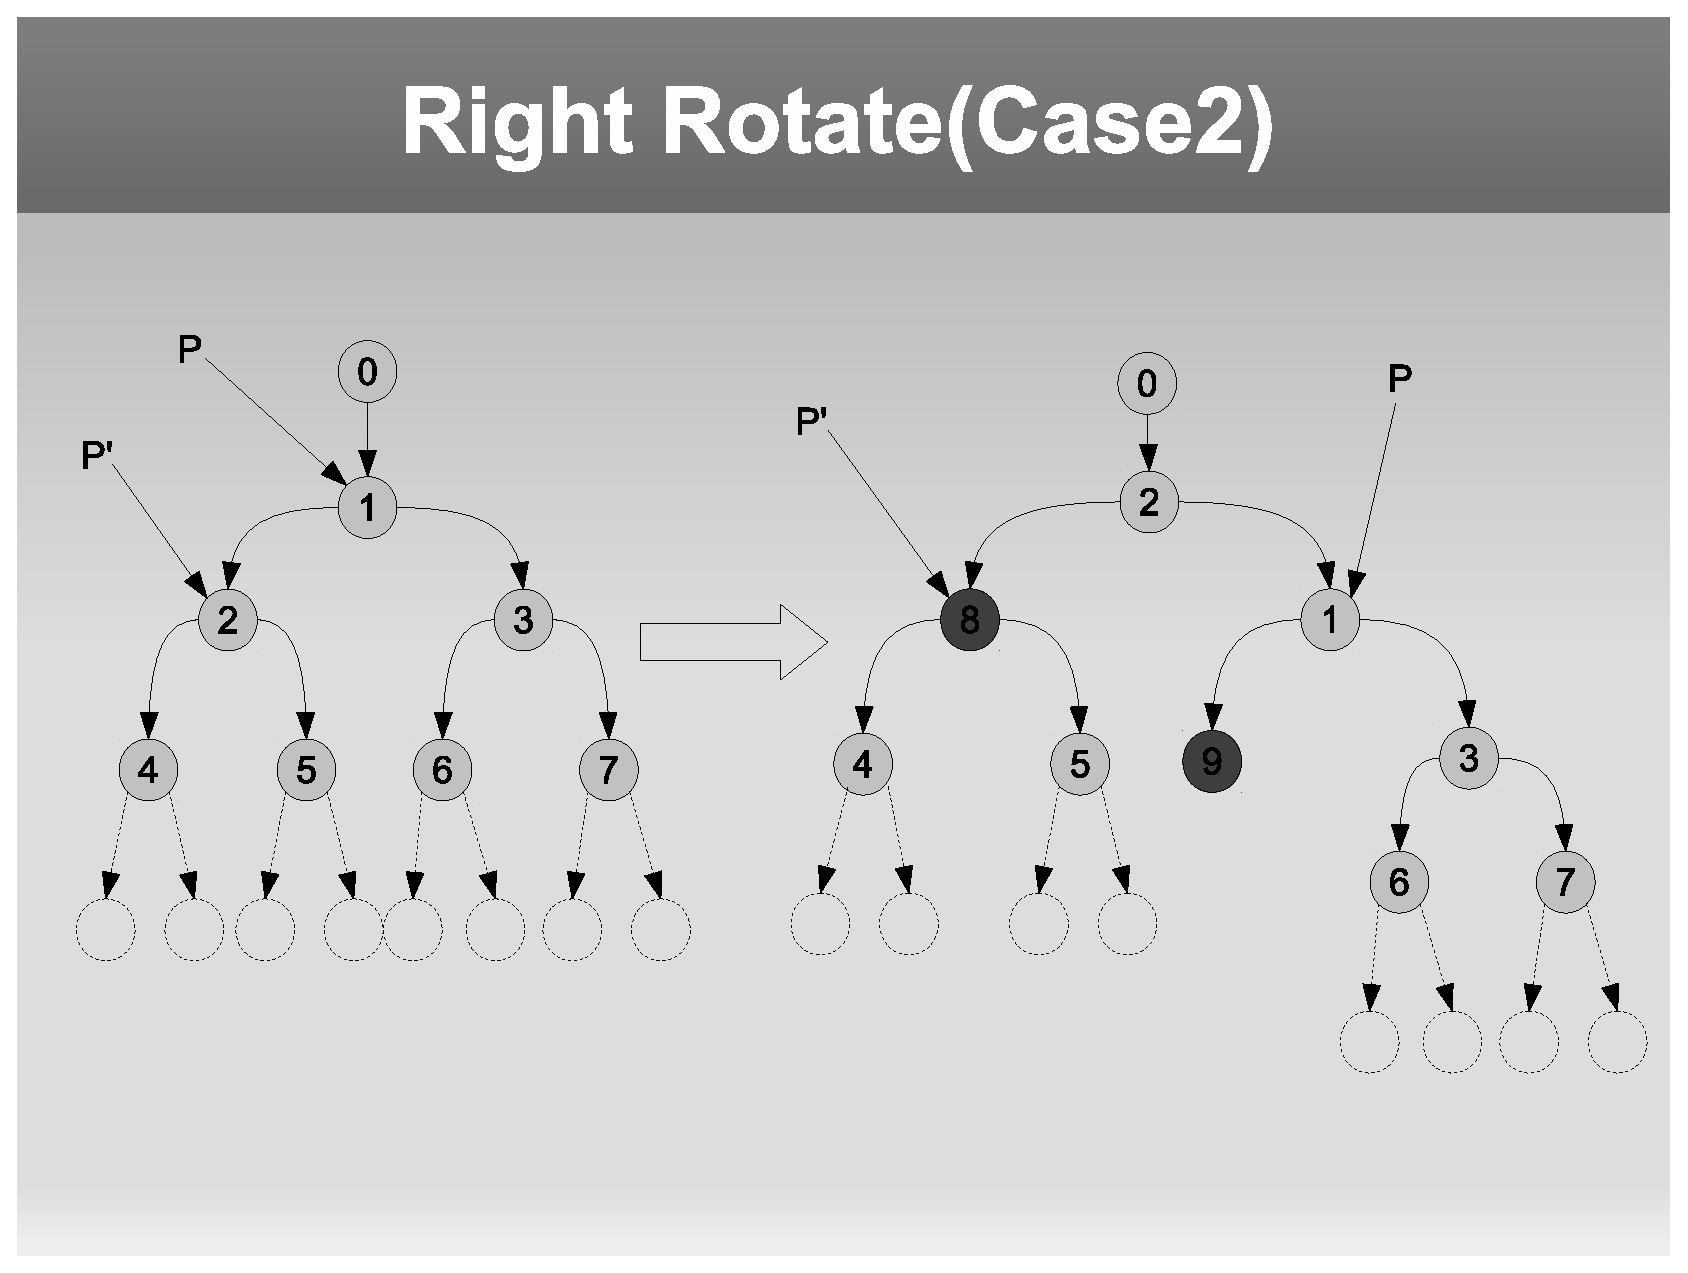
\includegraphics[scale=0.5]{right_rotate_2.eps}
    \caption{Right Rotate Case 2}
\end{figure}

\begin{figure}
    \centering
    \includegraphics[scale=0.5]{right_rotate_3.eps}
    \caption{Right Rotate Case 3}
\end{figure}

\begin{figure}
    \centering
    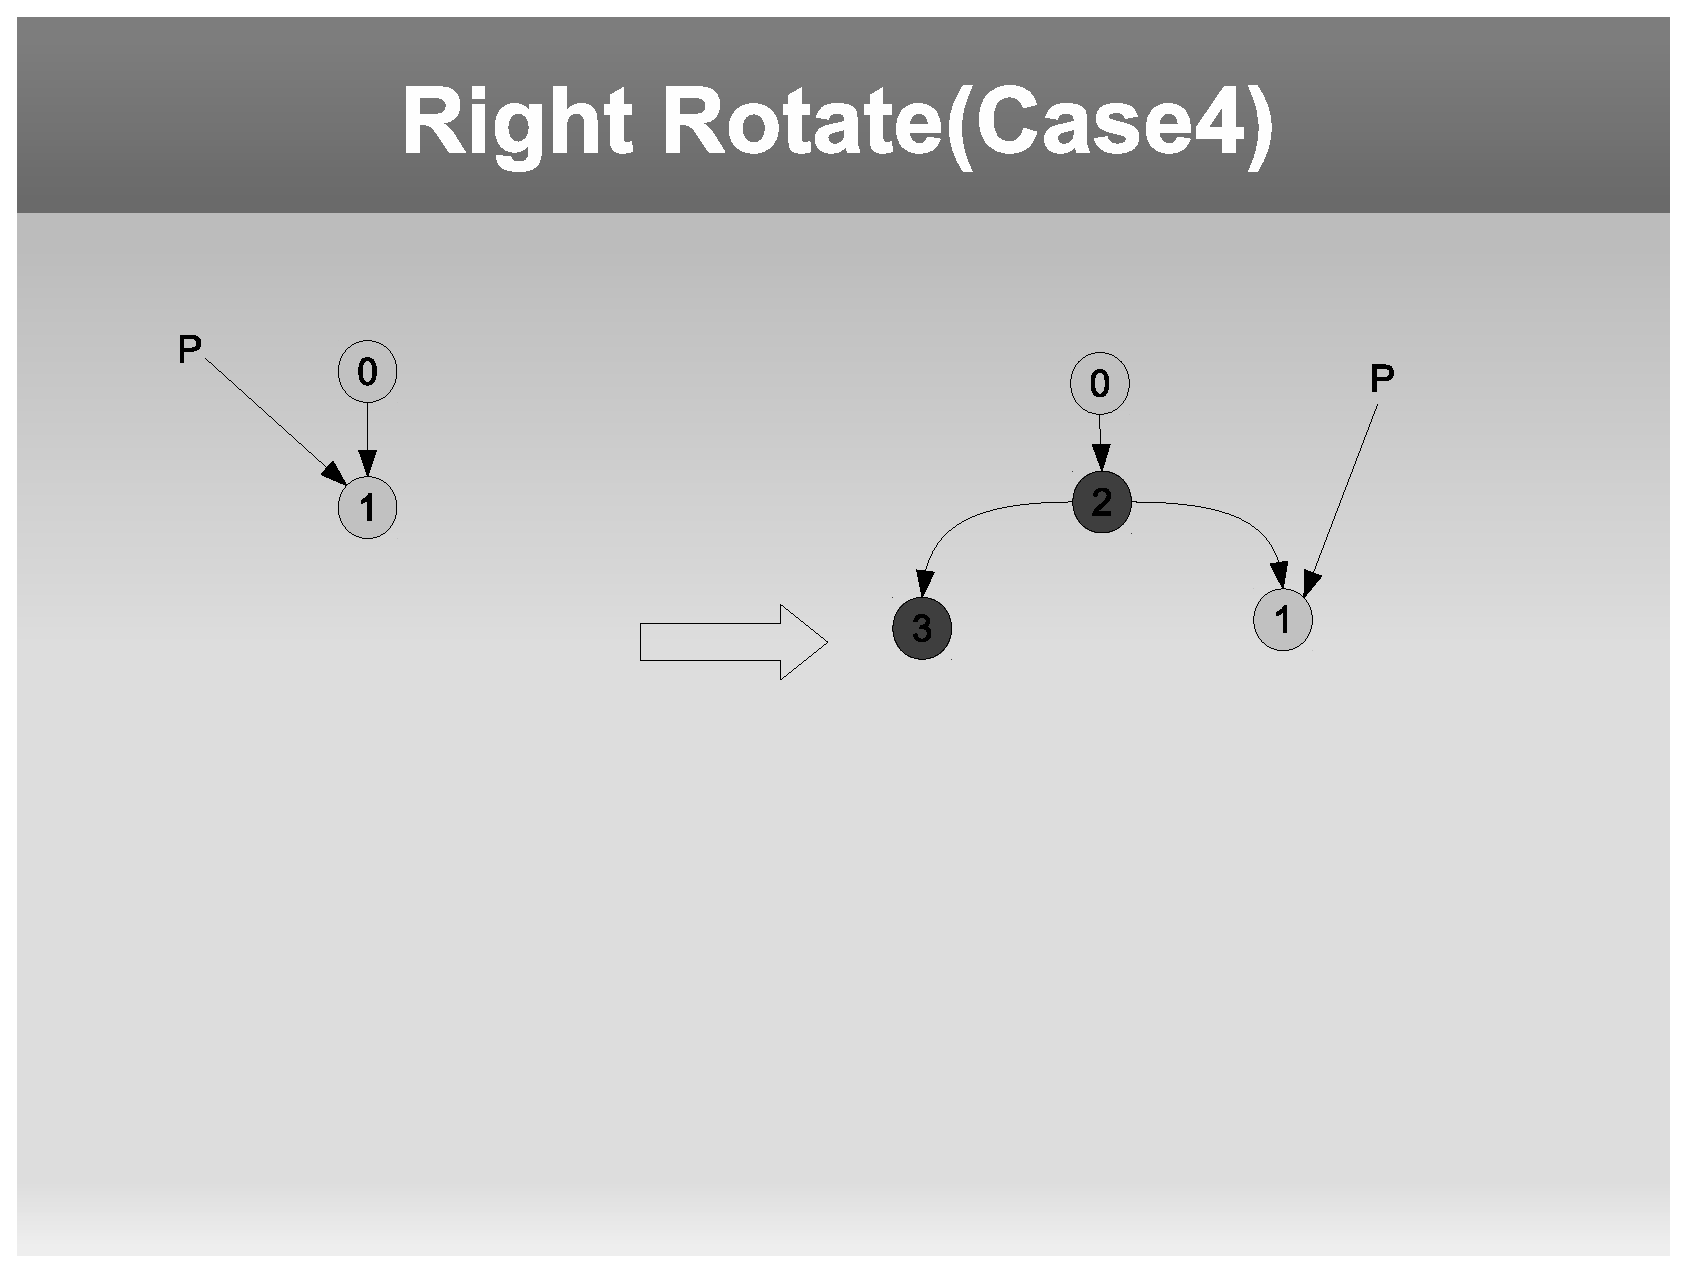
\includegraphics[scale=0.5]{right_rotate_4.eps}
    \caption{Right Rotate Case 4}
\end{figure}
\end{document}


